\documentclass[tikz,border=10pt]{standalone}
\usepackage{tikz}
\usetikzlibrary{shapes.geometric, arrows.meta, positioning, fit, shadows}

% Define colors
\definecolor{actorcolor}{RGB}{52, 73, 94}
\definecolor{usecasecolor}{RGB}{41, 128, 185}
\definecolor{admincolor}{RGB}{192, 57, 43}
\definecolor{bordercolor}{RGB}{149, 165, 166}

\begin{document}

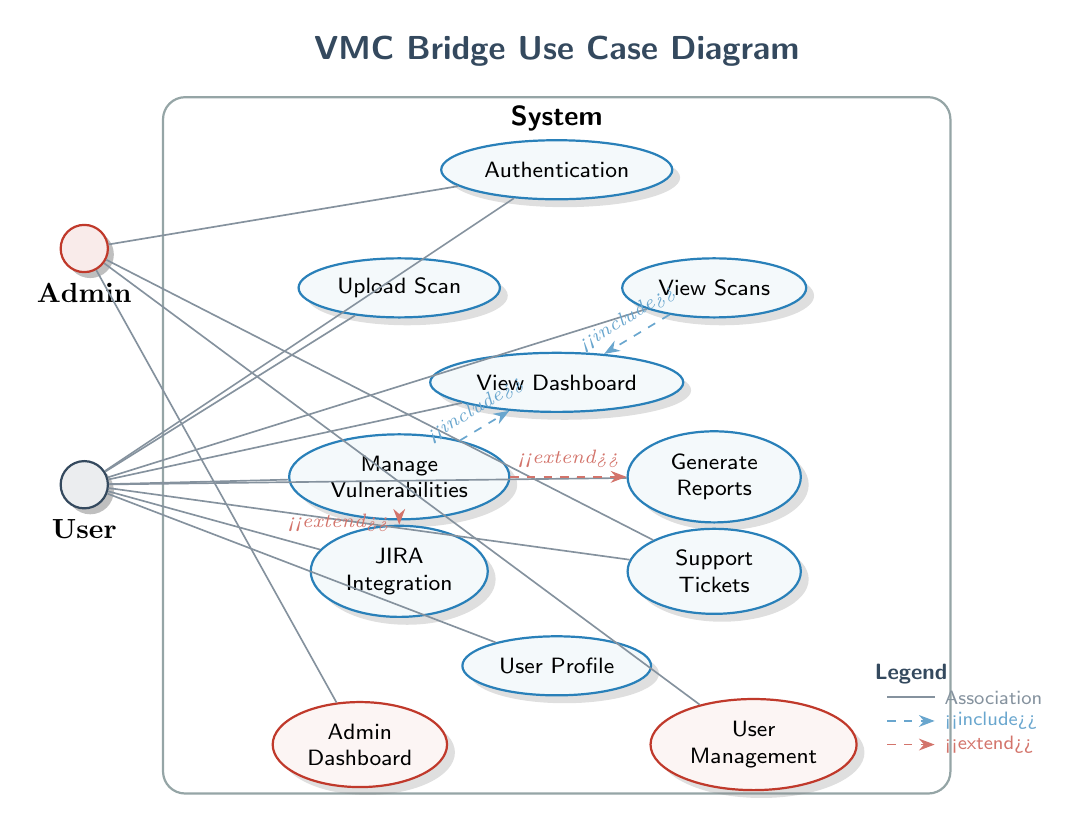
\begin{tikzpicture}[
    actor/.style={
        draw=actorcolor,
        fill=actorcolor!10,
        thick,
        circle,
        minimum size=0.6cm,
        font=\footnotesize\sffamily,
        drop shadow
    },
    usecase/.style={
        draw=usecasecolor,
        fill=usecasecolor!5,
        thick,
        ellipse,
        minimum width=2.2cm,
        minimum height=0.75cm,
        align=center,
        font=\footnotesize\sffamily,
        drop shadow={shadow xshift=0.1cm, shadow yshift=-0.1cm, opacity=0.25}
    },
    admincase/.style={
        draw=admincolor,
        fill=admincolor!5,
        thick,
        ellipse,
        minimum width=2.2cm,
        minimum height=0.75cm,
        align=center,
        font=\footnotesize\sffamily,
        drop shadow={shadow xshift=0.1cm, shadow yshift=-0.1cm, opacity=0.25}
    },
    include/.style={
        ->,
        >=Stealth,
        dashed,
        semithick,
        color=usecasecolor!70
    },
    extend/.style={
        ->,
        >=Stealth,
        dashed,
        semithick,
        color=admincolor!70
    },
    association/.style={
        -,
        semithick,
        color=actorcolor!60
    },
    boundary/.style={
        draw=bordercolor,
        thick,
        rounded corners=8pt,
        inner sep=12pt
    }
]

% Title
\node[font=\large\sffamily\bfseries, color=actorcolor] at (0, 9) {VMC Bridge Use Case Diagram};

% Actors
\node[actor, label=below:\textbf{User}] (user) at (-6, 3.5) {};
\node[actor, label=below:\textbf{Admin}, fill=admincolor!10, draw=admincolor] (admin) at (-6, 6.5) {};

% System boundary
\node[boundary, fit={(0, 0) (0, 8)}, minimum width=10cm, minimum height=8.5cm, 
      label={[anchor=north, font=\sffamily\bfseries]above:System}] (systembox) {};

% ==================== AUTHENTICATION ====================
\node[usecase] (auth) at (0, 7.5) {Authentication};

% ==================== USER USE CASES ====================
\node[usecase] (upload) at (-2, 6) {Upload Scan};
\node[usecase] (viewscan) at (2, 6) {View Scans};
\node[usecase] (dashboard) at (0, 4.8) {View Dashboard};
\node[usecase] (vuln) at (-2, 3.6) {Manage\\Vulnerabilities};
\node[usecase] (report) at (2, 3.6) {Generate\\Reports};
\node[usecase] (jira) at (-2, 2.4) {JIRA\\Integration};
\node[usecase] (support) at (2, 2.4) {Support\\Tickets};
\node[usecase] (profile) at (0, 1.2) {User Profile};

% ==================== ADMIN USE CASES ====================
\node[admincase] (adminpanel) at (-2.5, 0.2) {Admin\\Dashboard};
\node[admincase] (usermgmt) at (2.5, 0.2) {User\\Management};

% ==================== ASSOCIATIONS - USER ====================
\draw[association] (user) -- (auth);
\draw[association] (user) -- (upload);
\draw[association] (user) -- (viewscan);
\draw[association] (user) -- (dashboard);
\draw[association] (user) -- (vuln);
\draw[association] (user) -- (report);
\draw[association] (user) -- (jira);
\draw[association] (user) -- (support);
\draw[association] (user) -- (profile);

% ==================== ASSOCIATIONS - ADMIN ====================
\draw[association] (admin) -- (auth);
\draw[association] (admin) -- (adminpanel);
\draw[association] (admin) -- (usermgmt);
\draw[association] (admin) -- (support);

% ==================== RELATIONSHIPS ====================
\draw[include] (vuln) -- (dashboard) node[midway, above, sloped, font=\scriptsize\itshape] {<<include>>};
\draw[include] (viewscan) -- (dashboard) node[midway, above, sloped, font=\scriptsize\itshape] {<<include>>};
\draw[extend] (vuln) -- (jira) node[midway, left, font=\scriptsize\itshape] {<<extend>>};
\draw[extend] (vuln) -- (report) node[midway, above, sloped, font=\scriptsize\itshape] {<<extend>>};

% Legend
\begin{scope}[shift={(4.5, 0.5)}]
    \node[font=\footnotesize\sffamily\bfseries, color=actorcolor] at (0, 0.6) {Legend};
    \draw[association] (-0.3, 0.3) -- (0.3, 0.3) node[right, font=\scriptsize\sffamily] {Association};
    \draw[include] (-0.3, 0) -- (0.3, 0) node[right, font=\scriptsize\sffamily] {<<include>>};
    \draw[extend] (-0.3, -0.3) -- (0.3, -0.3) node[right, font=\scriptsize\sffamily] {<<extend>>};
\end{scope}

\end{tikzpicture}

\end{document}
